%----------------------------------------------------%
%                GESTION DEL PROYECTO                %
%----------------------------------------------------%

\chapter{Gestión del proyecto}
\label{gestion}

Añadir introducción.\\

\section{Metología Ágil}
\label{metodologia-agil}

Las metodologías ágiles son procesos para el desarrollo de software. Se basan en el desarrollo incremental e iterativo, donde varios grupos se unen para dar requerimientos y soluciones nuevas gracias a su colaboración. Se enfatiza en el cara a cara más que en la documentación. Un ejemplo de esta metodología es SCRUM.\\

La metodología es bastante flexible, pudiendo adaptarse a cada proyecto. Es decir, no tiene reglas absolutamente fijas. En su base esta el \textit{Manifiesto Ágil} en el que se basan todas las variantes de esta metodología. Este manifiesto \hyperref[manifiesto-agil]{\ref*{manifiesto-agil}} dice así:

\begin{itemize}
\item Individuos e interacciones sobre procesos y herramientas
\item Software funcionando sobre documentación extensiva
\item Colaboración con el cliente sobre negociación contractual
\item Respuesta ante el cambio sobre seguir un plan
\end{itemize}

\begin{quote}
\small Esto es, aunque valoramos los elementos de la derecha, valoramos más los de la izquierda.
\end{quote}

Al comienzo del proyecto se fijó el uso de esta metodología, con 4 grupos trabajando en paralelo (los equipos vienen definidos en el apartado \ref{equipos}). Sin embargo, las iteraciones acabaron volviéndose excesivamente largas, habiendo varios grupos parados. Si bien se respetó la filosofía de la metodología ágil en cierto sentido, y aun con cierta flexibilidad en su adaptación, al final del proyecto acabó por volverse algo parecido a una metodología ágil sin llegar a serlo.\\

\section{Metología InterMod}
\label{intermod}

InterMod es una metodología de trabajo, que será utilizada para este proyecto, desarrollada por el grupo de investigación GaLan de la Facultad de Informática de San Sebastián. Se trata una metodología ágil de desarrollo de alta calidad de software interactivo, incluyendo aplicaciones web.\\

En InterMod se define el Objetivo de Usuario (User Objetive o UO) como el deseo del usuario que puede ser alcanzado mediante una o más funcionalidades. Diferentes UOs son desarrollados durante el proyecto y la unión de todos, en su globalidad, forma la aplicación final. Además, el mismo UO puede estar incluido en uno o más requerimentos funcionales y/o no-funcionales. Existen a su vez diferentes tipos de UO:

\begin{itemize}
\item \textbf{UO Directo:} Es un objetivo del usuario final.
\item \textbf{UO Indirecto:} Surge a partir de otros UOs por necesidades interna del desarrollo (no son propiamente deseos del usuario). Aparecen durante el desarrollo debido a la fusión o división de otros UOs.
\item \textbf{UO Reutilizable:} Es un UO creado y evaluado, total o parcialmente, en otro proyecto o en el proyecto actual que puede ser reutilizado.
\end{itemize}

Basándose en la propuesta del Object Managemente Group’s Model Driven Architecture, Intermod establece sus actividades basadas en modelos.\\

Por cada actividad se desarrollan siempre dos fases: la creación del modelo (independiente de la plataforma) y su posterior evaluación. Las evaluaciones de usabilidad son especialmente útiles para los UOs Directos ya que reflejan una necesidad del usuario, por tanto es importante que un grupo de estos esté involucrado. Para agilizar el proyecto, algunos modelos pueden ser evaluados únicamente por expertos en usabilidad. Las actividades no se dan por acabadas y pueden continuar activas durante varias iteraciones hasta conseguir una evaluación positiva.\\

Existen dos tipos de actividades para el desarrollo de UOs: Actividades de Desarrollo (DA) y Actividades de Integración (IA). Existen tres tipos de DAs:

\begin{itemize}
\item \textbf{DA-1:} \textit{Análisis y Diseño de la Navegación.}
\item \textbf{DA-2:} \textit{Construcción de la Interfaz.}
\item \textbf{DA-3:} \textit{Codificación de la Lógica de Negocio.}
\end{itemize}

Para asegurar el desarrollo incremental de la aplicación son necesarias las Actividades de Integración (IA). Existen tres tipos de IAs:
\begin{itemize}
\item \textbf{IA-1:} \textit{Integración de los Modelos de Requerimientos.}
\item \textbf{IA-2:} \textit{Integración de la Interfaz.}
\item \textbf{IA-3:} \textit{Integración de la codificación y refactorización.}
\end{itemize}

Las actividades de desarrollo e integración de cada tipo da lugar a un modelo. Así, las DA-1 y IA-1, relativas al análisis de requisitos, desembocan en el modelo de requisitos (M-1); las DA-2 y IA-2, relativas a las interfaces, crean el modelo de presentación (M-2) y las DA-3 y IA-3, las asociadas a la lógica de negocio, constituyen el modelo de funcionalidad (M-3). El modelo M-1 es un modelo abstracto sobre el que se asientan las bases, basado en él se forma el M-2, que contiene todos los elementos gráficos y otras características definidos en el M-1. Finalmente el modelo M-3 establece la implementación en un lenguaje de programación concreto.\\

InterMod define una metodología dividida en iteraciones, y, a diferencia del resto, define un paso previo, Step 0. En esta etapa previa se realiza el análisis del proyecto y se definen los UOs iniciales del mismo y el diseño general. A continuación se pasa a la iteración 1, luego la 2, etc. y se continúa así hasta dar por finalizado el proyecto. Cada iteración esta dividida en 3 pasos:

\begin{itemize}
\item \textbf{Step 1.i:} Construir/Actualizar la lista de UOs.
\item \textbf{Step 2.i:} Planificar las actividades para los diferentes equipos.
\item \textbf{Step 3.i:} Realizar las actividades planificadas.
\end{itemize}

\subsection{Adaptación de InterMod}
\label{adaptacion-intermod}

Debido a las características del proyecto se ha decidido realizar algunas modificaciones al esquema de InterMod:

\begin{itemize}
\item Los UOs normalmente se denotan por UOX (siendo X el número del UO). En este proyecto hemos distinguido dos usuarios, por tanto hará falta un identificador extra para saber a que usuario corresponde el UO. Se usará la notación UOX-Y, siendo Y la inicial en inglés del tipo de usuario: 'S' para el estudiante (\textit{Student}) y 'T' para el profesor (\textit{Teacher}).
\item Siguiendo la línea del punto anterior, se ha hecho un cambio en la notación típica de los modelos. De M-1(X), el primer modelo del UOX, a M-1(XY), el primer modelo del UOX-Y (siguiendo la notación del punto anterior).
\end{itemize}

\section{Formación de equipos}
\label{equipos}

Se han identificado 4 equipos que participarán en el proyecto (interesados en el proyecto):

\begin{itemize}
\item \textbf{Equipo 1:} Formado por el alumno, Adrián Núñez. Se encargará del diseño de las interfaces y de la implementación de la aplicación.
\item \textbf{Equipo 2:} Realizara las evaluaciones pertinentes y estará formado por alumnos de la facultad.
\item \textbf{Equipo 3:} Segundo equipo para las evaluaciones, estará formado por miembros del grupo GaLan.
\item \textbf{Equipo 4:} Se encargará de las evaluaciones con los usuarios finales.
\end{itemize}

\section{Canales de comunicación e Infraestructura de almacenamiento}

Con el fin de mantener la comunicación con los interesados en el proyecto se plantea el canal de comunicación \textit{Slack} (https://slack.com/) al inicio del proyecto. Mediante este canal se intercambiaran mensajes rápidos entre  y Adrián Núñez para cualquier duda u opinión rápida.\\

También se realizaran periódicamente reuniones presenciales, como mínimo, entre Maite Urretavizcaya y Adrián Núñez para monitorizar el desarrollo del proyecto. A estas reuniones también han asistido Samara Ruíz (en su mayoría) y Juan Miguel López.\\

Para la comunicación con el Equipo 2 se utilizó la herramienta de mensajería móvil \textit{Telegram} (que permite, al contrario que otras conocidas, el intercambio de cualquier tipo de fichero, vital para pasarles el fichero .apk).\\

Finalmente, el proyecto y este documento estarán públicos en \textit{GitHub} en el siguiente repositorio: https://github.com/AdrianNunez/exerClick. Se realizaran periódicamente actualizaciones del mismo. También se dispone de otras copias en el ordenador personal del autor, Adrián Núñez, y en el espacio de almacenamiento \textit{Google Drive}, en una carpeta compartida con Maite Urretavizcaya y Samara Ruíz.\\

\section{Sistemas Operativos evaluados}
\label{sistemas-operativos}

En la propia documentación de Apache Cordova vienen indicados los Sistemas Operativos soportados a los que se puede adaptar la aplicación:

\begin{itemize}
\item iOS (Mac)
\item Amazon Fire OS (Mac, Linux, Windows)
\item Android (Mac, Linux, Windows)
\item BlackBerry 10 (Mac, Linux, Windows)
\item Windows Phone 8 (Windows)
\item Windows (Windows)
\item Firefox OS (Mac, Linux, Windows)
\end{itemize}

Ya que el abanico de posibilidades es extenso se decidió reducir las posibilidades a iOS, Android, BlackBerry 10 y Windows Phone 8. El desarrollo principal y todas las pruebas iniciales se realizarán utilizando Android.\\

Al final del proyecto, debido a incompatibilidades con la infraestructura disponible, se realizaron sólo evaluaciones en dispositivos fisicos Android e iOS.\\

\section{Tecnologías y Herramientas utilizadas}
\label{tecnologias}

Al inicio, antes del desarrollo de la aplicación, se concretaron las siguientes tecnologías mínimas a utilizar:

\begin{itemize}
\item HTML5
\item CSS3
\item PHP
\item MySQL
\end{itemize}

Como calidad añadida se utilizan las siguientes tecnologías:

\begin{itemize}
\item Javascript
\item JQuery
\end{itemize}

Las herramientas principales para el desarrollo de la aplicación serán Notepad++ y Eclipse. Para la gestión de la base de datos se usará phpMyAdmin y para la gestión del servidor se usará WinSCP.\\

Para el desarrollo en Android se utilizará la SDK de Android y el emulador Genymotion (mucho más rápido que el emulador por defecto).\\

%----------------------------------------------------%
%               	    STEP 0                       %
%----------------------------------------------------%

\section{Step 0 - Análisis del proyecto}
\label{step0}

\begin{flushleft}
\textbf{Fecha de inicio:} 9/10/14\\
\textbf{Fecha de fin:} 18/10/14\\
\textbf{Dedicación total:} 2 horas, 35 minutos\\
\end{flushleft}

Esta fase previa al desarrollo de la aplicación principal se planteó dentro de la metodología InterMod como una introducción. En este proyecto se realizaron dos tareas principalmente:

\begin{itemize}
\item Documentarse sobre el estado del arte en el ámbito de aplicaciones de seguimiento de ejercicios en el aula, sobre bases de datos que representaran el concepto de ejercicio, etc.
\item Realizar un \textit{Brainstorming} para plantear todas las ideas posibles para la aplicación. De esta forma se pretender tener una idea más clara de como será la aplicación que se desea.
\end{itemize}

Finalmente se realizó la lista de UOs inicial que incluía muchos UOs no prioritarios. Sin embargo, se decidió dejar la lista completa e ir abordándola por prioridades y actualizándola iteración por iteración.\\

\subsection{UOs inicialmente planteados}
\label{step0:uos}

\textbf\textit{\large UOs del alumno}\\

\colorbox{YellowGreen}{\parbox[c]{1.0\textwidth}{
	\textbf{UO1-S:} \textit{Responder a un ejercicio.} El alumno quiere indicar que ha acabado o que tiene dudas con 			un ejercicio que el profesor ha propuesto.\\
}}\\

\vspace{0.3cm}

\textbf\textit{\large UOs del profesor}\\

\colorbox{SkyBlue}{\parbox[c]{1.0\textwidth}{
\textbf{UO1-T:} \textit{Crear-lanzar un ejercicio simple.} El profesor quiere proponer un ejercicio rápidamente, sin escribir mucho.\\
}}\\

\vspace{0.1cm}

\colorbox{SkyBlue}{\parbox[c]{1.0\textwidth}{
\textbf{UO2-T:} \textit{Crear-lanzar un ejercicio detallado.} El profesor quiere proponer la realización de un ejercicio preparado previamente o con bastantes detalles.\\
}}\\

\vspace{0.1cm}

\colorbox{SkyBlue}{\parbox[c]{1.0\textwidth}{
\textbf{UO3-T:} \textit{Dar por finalizado un ejercicio propuesto activo.} El profesor quiere terminar con uno de los ejercicios que propuso.\\
}}\\

\vspace{0.1cm}

\colorbox{SkyBlue}{\parbox[c]{1.0\textwidth}{
\textbf{UO4-T:} \textit{Ver estadísticas de un ejercicio.} El profesor desea ver qué tal le ha ido a la clase en general o a un alumno en un ejercicio.\\
}}\\

\vspace{0.1cm}

\colorbox{SkyBlue}{\parbox[c]{1.0\textwidth}{
\textbf{UO5-T:} \textit{Ver la descripción completa de un ejercicio.} Un profesor quiere ver la descripción completa de un ejercicio (identificador, enunciado, página, tema, etc.).\\
}}\\

\vspace{0.1cm}

\colorbox{SkyBlue}{\parbox[c]{1.0\textwidth}{
\textbf{UO6-T:} \textit{Editar un ejercicio.} El profesor desea editar los atributos de un ejercicio.\\
}}\\

\vspace{0.1cm}

\colorbox{SkyBlue}{\parbox[c]{1.0\textwidth}{
\textbf{UO7-T:} \textit{Evaluar el ejercicio de un alumno.} El profesor quiere valorar la realización de un ejercicio a un alumno.\\
}}\\

\vspace{0.1cm}

\colorbox{SkyBlue}{\parbox[c]{1.0\textwidth}{
\textbf{UO8-T:} \textit{Cerrar sesión.} El profesor quiere cerrar su sesión activa.\\
}}\\

\vspace{0.1cm}

\colorbox{SkyBlue}{\parbox[c]{1.0\textwidth}{
\textbf{UO9-T:} \textit{Cambiar el idioma de la aplicación.} El profesor desea cambiar el idioma con el que lee la aplicación.\\
}}\\

\vspace{0.1cm}

\colorbox{SkyBlue}{\parbox[c]{1.0\textwidth}{
\textbf{UO10-T:} \textit{Cambiar de asignatura.} El profesor, que tiene más de una asignatura, quiere cambiar de una asignatura x a otra asignatura y.\\
}}\\

%----------------------------------------------------%
%                     ITERACION 1                    %
%----------------------------------------------------%

\section{Iteración 1}
\label{it1}

\begin{flushleft}
\textbf{Fecha de inicio:} 21/10/14\\
\textbf{Fecha de fin:} 2/11/14\\
\textbf{Dedicación total:} 3 horas, 25 minutos\\
\end{flushleft}

\subsection{Step 1.1. Lista de UOs}
\label{it1:1.1}

Debido a la gran cantidad de UOs planteados se ha decidido seleccionar los considerados como prioritarios. En esta primera etapa se quieren desarrollar los que creemos que son los más importantes:

\begin{itemize}
\item UOs del alumno:
	\begin{itemize}
	\item \textbf{UO1-S:} \textit{Responder a un ejercicio.}
	\end{itemize}
\item UOs del profesor:
	\begin{itemize}
	\item \textbf{UO1-T:} \textit{Crear-lanzar un ejercicio simple.}
	\item \textbf{UO2-T:} \textit{Crear-lanzar un ejercicio detallado.}
	\item \textbf{UO3-T:} \textit{Dar por finalizado un ejercicio propuesto activo.}
	\item \textbf{UO4-T:} \textit{Ver estadísticas de un ejercicio.}
	\end{itemize}
\end{itemize}

\subsection{Step 2.1. Planificación de la iteración}
\label{it1:2.1}

En esta primera iteración el plan es el siguiente:

\begin{itemize}
\item Equipo 1: M-1 de todos los UOs iniciales
\item Equipo 3: Evaluación{M-1 de todos los UOs iniciales}
\end{itemize}

\subsection{Step 3.1. Ejecución de las actividades}
\label{it1:3.1}

Con la síntesis de lo acordado en la última reunión se modifica el documento de Brainstorming, que queda corregido para tener todas las ideas previas claras por escrito.\\

Se empiezan realizando los M-1 (prototipos de papel) de los UOs planteados inicialmente (de la lista entera). Los prototipos en papel se envían durante la iteración a Maite y Samara para valoraciones rápidas y posteriores correcciones.\\

%----------------------------------------------------%
%                     ITERACION 2                    %
%----------------------------------------------------%

\section{Iteración 2}
\label{it2}

\begin{flushleft}
\textbf{Fecha de inicio:} 3/11/14\\
\textbf{Fecha de fin:} 10/11/14\\
\textbf{Dedicación total:} 3 horas, 30 minutos\\
\end{flushleft}

\subsection{Step 1.2. Lista de UOs}
\label{it2:1.2}

Lista de UOs = {UO1-T, UO2-T, UO3-T, UO4-T}

\subsection{Step 2.2. Planificación de la iteración}
\label{it2:2.2}

Se continúa con el mismo plan de la pasada iteración.

\begin{itemize}
\item Equipo 1: M-1 de todos los UOs iniciales
\item Equipo 3: Evaluación{M-1 de todos los UOs iniciales}
\end{itemize}

\subsection{Step 3.2. Ejecución de las actividades}
\label{it2:3.2}

Se corrigen los prototipos en papel con lo acordado durante la pasada reunión y se realizan nuevos a limpio.\\

%----------------------------------------------------%
%                     ITERACION 3                    %
%----------------------------------------------------%

\section{Iteración 3}
\label{it3}

\begin{flushleft}
\textbf{Fecha de inicio:} 11/11/14\\
\textbf{Fecha de fin:} 12/1/15\\
\textbf{Dedicación total:} 72 horas, 55 minutos\\
\end{flushleft}

\subsection{Step 1.3. Lista de UOs}
\label{it3:1.3}

Lista de UOs = {UO1-T, UO2-T, UO3-T, UO4-T}

\subsection{Step 2.3. Planificación de la iteración}
\label{it2:2.3}

\begin{itemize}
\item Equipo 1: UO1-T[M-2]
\end{itemize}

\subsection{Step 3.3. Ejecución de las actividades}
\label{it2:3.3}

Durante esta iteración se instala el entorno de trabajo de Cordova. Se instalan inicialmente las plataformas Android y Windows Phone. Se decide también iniciar todas las pruebas utilizando Android.\\

Se comienza con el M-2 del UO1-T, que servirá como base para otros UOs (ya que casi todos comparten la pantalla madre que se desarrolla en esta fase).\\

El proyecto queda exportado a Eclipse para intentar generar el fichero .apk de modo que cualquiera pueda probar la aplicación, aunque no se consigue que este funcione. Queda pendiente para una futura iteración.\\

También se fija que la versión de Android mínima para utilizar la aplicación sin problema es la 3.0.\\

%----------------------------------------------------%
%                     ITERACION 4                    %
%----------------------------------------------------%

\section{Iteración 4}
\label{it4}

\begin{flushleft}
\textbf{Fecha de inicio:} 13/1/15\\
\textbf{Fecha de fin:} 26/1/15\\
\textbf{Dedicación total:} 16 horas\\
\end{flushleft}

\subsection{Step 1.4. Lista de UOs}
\label{it4:1.4}

Lista de UOs = {UO1-T, UO2-T, UO3-T, UO4-T, UO1-S}

\subsection{Step 2.4. Planificación de la iteración}
\label{it4:2.4}

\begin{itemize}
\item Equipo 1: UO1-T[M-2], UO4-T[M-2], UO1-S[M-2]
\end{itemize}

\subsection{Step 3.4. Ejecución de las actividades}
\label{it4:3.4}

Se añaden las correcciones acordadas en la anterior reunión al M-2 del UO1-T y se inician en esta fase los M-2 de los UO4-T y UO1-S. También se sube el proyecto a GitHub para el control de versiones y tener una copia de seguridad extra.\\

Más avanzados en la iteración se le ha proporcionado al alumno la base de datos de PreseceClick vacía para poder empezar con la lógica de negocio o el M-3 de los UOs realizados. Se han creado dos tablas nuevas exclusivas para exerClick:

\begin{itemize}
\item \textbf{exercise:} Almacena información sobre un ejercicio.
\item \textbf{exercisestate:} Almacena el estado de un ejercicio.
\end{itemize}

%----------------------------------------------------%
%                     ITERACION 5                    %
%----------------------------------------------------%

\section{Iteración 5}
\label{it5}

\begin{flushleft}
\textbf{Fecha de inicio:} 27/1/15\\
\textbf{Fecha de fin:} 6/2/15\\
\textbf{Dedicación total:} 23 horas, 15 minutos\\
\end{flushleft}

\subsection{Step 1.5. Lista de UOs}
\label{it5:1.5}

Lista de UOs = {UO1-T, UO2-T, UO3-T, UO4-T, UO1-S}

\subsection{Step 2.5. Planificación de la iteración}
\label{it5:2.5}

\begin{itemize}
\item Equipo 1: UO1-T[M-3], UO3-T[M-2,M-3], UO4-T[M-3], UO1-S[M-3]
\item Equipo 3: Evaluación{UO1-T[M-2], UO3-3[M-2], UO4-T[M-2]}
\end{itemize}

\subsection{Step 3.5. Ejecución de las actividades}
\label{it5:3.5}

Se empieza la iteración modificando el aspecto de la pantalla madre (correspondiente a casi todos los UOs del docente).\\

Para pasar la aplicación al móvil es necesario que el código PHP (de servidor) este en un servidor externo, de otro modo no funcionara. Se ha creado para ese propósito un servidor con el espacio que proporciona 000webhost (http://www.000webhost.com/) sin costo alguno para realizar pruebas al principio. Se ha instalado la base de datos proporcionada ahí mismo con las tablas originales más las dos creadas en la iteración anterior.\\

Se ha empezado realizando el M-3 del UO1-T, luego el UO4-T y finalmente el UO3-T. El objetivo de la iteración es tener una aplicación mínimamente funcional para realizar pruebas. Es decir, poder al menos realizar la función básica de que el profesor lance un ejercicio, el alumno lo vea y responda. Además, ver las estadísticas del ejercicio propuesto también sería importante.\\

Al abordar el UO3-T se han encontrado otros subobjetivos, derivados también de la reunión del día 27 de enero. En la reunión se decidió que los ejercicios, estuvieran en el estado que estuvieran (activos, finalizados o preparados para lanzarse), podrían cambiarse a cualquier estado. Es decir, el UO3-T tenía como objetivo el cambio de ejercicio activo a ejercicio finalizado, pero con esta decisión se deben de poder realizar cualquier otro cambio posible además del anterior.\\

\vspace{0.1cm}

\colorbox{SkyBlue}{\parbox[c]{1.0\textwidth}{
\textbf{UO3-T:} \textit{Cambiar el estado de un ejercicio.} El profesor quiere, por ejemplo, terminar con uno de los ejercicios que propuso o quiere volver a poner como activo un ejercicio que por error ha marcado como finalizado.\\
}}\\

\vspace{0.1cm}

En esta iteración no se ha implementado la identificación de usuarios, por lo que sigue estando como en la iteración previa.\\

Se ha ocultado la pestaña de ejercicios preparados hasta que se aborde el tema.\\

%----------------------------------------------------%
%                     ITERACION 6                    %
%----------------------------------------------------%

\section{Iteración 6}
\label{it6}

\begin{flushleft}
\textbf{Fecha de inicio:} 9/2/15\\
\textbf{Fecha de fin:} -\\
\textbf{Dedicación total:} - horas, - minutos\\
\end{flushleft}

\subsection{Step 1.6. Lista de UOs}
\label{it6:1.6}

Lista de UOs = {UO1-S, UO2-S, UO5-T, UO6-T, UO8-T, UO9-T, UO10-T}

\subsection{Step 2.6. Planificación de la iteración}
\label{it6:2.6}

\begin{itemize}
\item Equipo 1: UO1-T[M-3], UO2-T[M-2,M-3], UO3-T[M-3], UO4-T[M-3], UO1-S[M-3], UO2-S[M-2,M-3], UO5-T[M-2,M-3], UO6-T[M-2,M-3], UO7-T[M-2,M-3], UO9-T[M-2,M-3]
\item Equipo 2: Evaluación de las .apks generadas durante el desarrollo
\item Equipo 3: Evaluación de las .apks generadas durante el desarrollo
\end{itemize}

\subsection{Step 3.6. Ejecución de las actividades}
\label{it6:3.6}

La iteración 6 se puede dividir en dos partes importantes: la primera en la que se crean los UOs restantes para tener una aplicación completamente funcional y la segunda en la que se genera finalmente un apk y se comienzan las pruebas.\\

Tras la reunión que daba inicio a esta iteración se realizaron todas las modificaciones y correcciones acordadas para empezar. El objetivo principal era completar el UO principal que forma el UO1-T, el UO1-S y el UO4-T (es decir, añadir ejercicios, responder a ellos y ver los resultados). Para ello primero había que convertir los datos estáticos en datos obtenidos de la base de datos (asignatura, estadísticas, etc.). Además de esto se realizaron muchísimas actividades más:

\begin{itemize}
\item Se creó el perfil para el profesor y el UO8-T (cerrar sesión) y el UO9-T (cambiar de asignatura).
\item Se probó por primera vez en una tablet la aplicación completa.
\item Se añadieron estadísticas diferentes para los ejercicios que estaban finalizados.
\item Se añadieron los ejercicios preparados.
\item Se modificó el funcionamiento de los botones para marcar el estado de un ejercicio en la vista del alumno.
\item Se realizaron pruebas con el Grupo 2, formado por alumnos, por primera vez.
\item Se añadió la opción de crear ejercicios avanzados.
\item UO5-T para ver detalles de un ejercicio y UO6-T para editar un ejercicio.
\end{itemize}

Para generar el fichero .apk se usó Eclipse Luna y Java 8. Se exportó el proyecto a Eclipse y se realizaron las configuraciones necesarias. Surgieron unas gran cantidad de errores que supusieron la mayor parte del tiempo de esta parte. Finalmente, cuando todo funcionaba correctamente y la aplicación se ejecutaba en el emulador, Eclipse generaba un fichero .apk correcto. Este fichero le fue pasado a Maite Urretavizcaya, Samara Ruíz y al Equipo 2 para realizar pruebas.\\

%----------------------------------------------------%
%      DOCUMENTACION DE LA GESTION DEL PROYECTO      %
%----------------------------------------------------%

\section{Documentación de la gestión del proyecto}
\label{dgp}

A continuación se presenta un resumen completo de los objetivos desarrollados en las iteraciones. Con el paso de estas los objetivos se han fusionado, divididos o han ido evolucionando. Estos procesos se muestran de manera gráfica para dar una visión rápida del origen de cada UO. En esta leyenda se muestran todos los UOs desarrollados:\\

\vspace{0.1cm}

\noindent
\framebox{\parbox[c]{1.0\textwidth}{
\textbf{Notación}\\

\textbf{UOX-Y:} UO Directo.\\
\textbf{\framebox{UOX-Y}:} UO por Fusión.\\
\textbf{\underline{UOX-Y}:} UO por División.\\
}}\\

\vspace{0.1cm}

\noindent
\framebox{\parbox[c]{1.0\textwidth}{
\textbf{Alumno}\\

\textbf{UO1-S:} \textit{Responder a un ejercicio.} El alumno quiere indicar que ha acabado o que tiene dudas con un ejercicio que el profesor ha propuesto.\\

\textbf{UO2-S:} \textit{Ver detalles de un ejercicio.} El alumno quiere ver más detalles sobre un ejercicio disponible y activo en la sesión.\\
}}\\

\vspace{0.1cm}

\noindent
\framebox{\parbox[c]{1.0\textwidth}{
\textbf{Profesor}\\

\textbf{UO1-T:} \textit{Crear-Lanzar un ejercicio simple.} El profesor quiere proponer un ejercicio rápidamente, sin escribir mucho.\\

\textbf{UO2-T:} \textit{Crear un ejercicio detallado.} El profesor quiere proponer la realización de un ejercicio preparado previamente o con bastantes detalles.\\

\textbf{UO3-T:} \textit{Cambiar el tipo de ejercicio.} El profesor desea cambiar un ejercicio del tipo que tiene a otro cualquiera (de activo a finalizado, por ejemplo).\\

\textbf{UO4-T:} \textit{El profesor desea ver qué tal le ha ido a la clase en general o a un alumno en un ejercicio.} El profesor desea ver qué tal le ha ido a la clase en general o a un alumno en un ejercicio.\\

\textbf{UO5-T:} \textit{Ver la descripción completa de un ejercicio.} Un profesor quiere ver la descripción completa de un ejercicio (identificador, enunciado, página, tema, etc.).\\

\textbf{UO6-T:} \textit{Editar un ejercicio.} El profesor desea editar los atributos de un ejercicio.\\

\textbf{UO8-T:} \textit{Cerrar sesión.} El profesor quiere cerrar su sesión activa.\\

\textbf{UO9-T:} \textit{Cambiar el idioma de la aplicación.} El profesor desea cambiar el idioma con el que lee la aplicación.\\

\textbf{UO10-T:} \textit{ Cambiar de asignatura.} El profesor, que tiene más de una asignatura, quiere cambiar de una asignatura x a otra asignatura y.\\

\textbf{\framebox{UO1}:} \textit{Lanzar ejercicios.} El profesor desea lanzar un ejercicio simple o avanzado, dependiendo de su necesidad.\\

\textbf{\framebox{UO2}:} \textit{Lanzar ejercicios y visualizar resultados.} El profesor desea lanzar un ejercicio y, tras lanzarlo, ver el estado de cada alumno en dicho ejercicio.\\
}}\\

\vspace{0.1cm}

\noindent
\framebox{\parbox[c]{1.0\textwidth}{
\textbf{Generales}\\

\textbf{\framebox{UO3}:} \textit{Lanzar ejercicios, responder al ejercicio y visualizar los resultados.} El profesor desea lanzar un ejercicio, el alumno desea responder al ejercicio y finalmente el profesor desea ver el estado de ese alumno en el ejercicio que ha lanzado previamente.\\
}}\\

\vspace{0.1cm}

Y los UOs definidos pero que no han sido realizados:\\

\vspace{0.1cm}

\noindent
\framebox{\parbox[c]{1.0\textwidth}{
\textbf{UO7-T:} \textit{Evaluar el ejercicio de un alumno.} El profesor quiere valorar la realización de un ejercicio a un alumno.\\
}}\\

\vspace{0.1cm}

\subsection{Selección de UOs por iteraciones}
\label{dgp:uos-iteraciones-creacion}

En la figura ~\ref{fig:grafico-seleccion-uos} se muestra el proceso de selección de UOs dividido por iteraciones. Con "seleccionar" se quiere decir que se añade a la planificación de la iteración para realizar alguno de los modelos del UO.

\begin{figure}[h]
	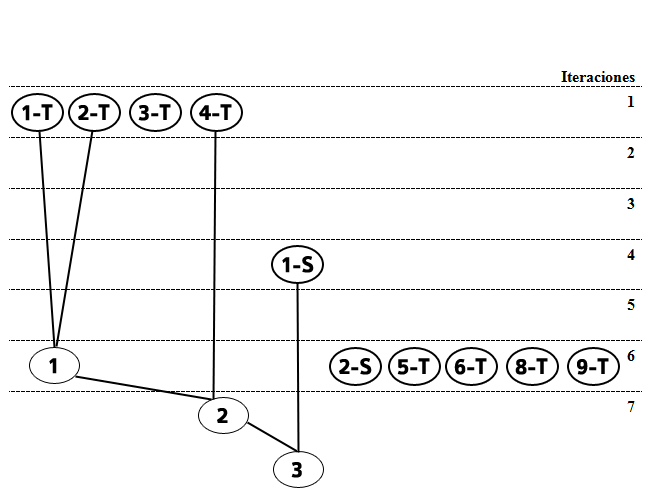
\includegraphics[width=\linewidth]{grafico-seleccion-uos}
	\caption{Progreso del proyecto según selección de UOs}
	\label{fig:grafico-seleccion-uos}
\end{figure}

Los UOs directos aparecen con un borde negro grueso y los UOs por Fusión con un borde negro simple. Las líneas que unen los UOs indican una relación de fusión.\\

\subsection{Desarrollo de actividades por iteraciones}
\label{dgp:desarrollo-actividades}

En la figura ~\ref{fig:grafico-desarrollo-actividades} se detalla el desarrollo de los diferentes tipos de actividad (de desarrollo o de integración) para cada UO en base a las iteraciones.

\begin{figure}[h]
	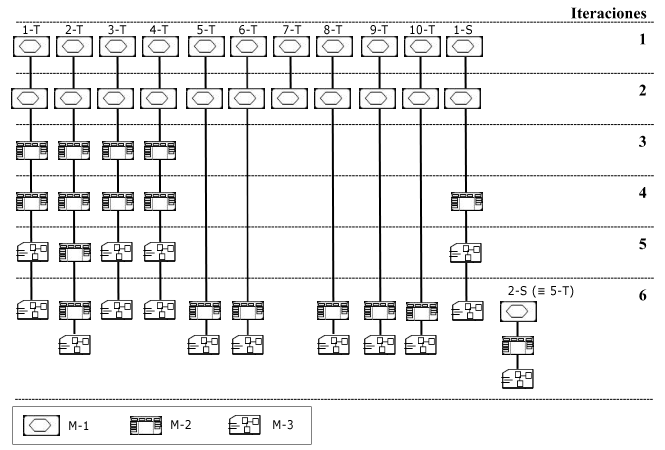
\includegraphics[width=\linewidth]{grafico-desarrollo-actividades}
	\caption{Progreso del proyecto según el desarrollo de Actividades}
	\label{fig:grafico-desarrollo-actividades}
\end{figure}

Las actividades se unen por líneas si estan relacionadas entre sí, estén o no en la misma iteración. Las líneas gruesas indican el flujo normal de desarrollo y las líneas delgadas el flujo de integración.\\

\subsection{Modelos evaluados por iteraciones}
\label{dgp:modelos-evaluados}

En la tabla \ref{table:tabla-progreso-modelos-evaluados} se pueden ver valores asociados a cada par de UO y modelo, estos valores siguen la notación:\\

\framebox{\parbox[c]{1.0\textwidth}{
Modelos obtenidos debido a una actividad o proceso:
\begin{itemize}
\item X: debido a una DA.
\item I: debido a una IA.
\item \underline{I}: debido a una Integración Incremental \underline{IA}.
\item D: derivado de un proceso de división de un UO.
\item F: derivado de un proceso de fusión de UOs.
\end{itemize}
El número expresa la iteración en la que se evaluó
satisfactoriamente dicho modelo.
}}\\

\noindent
\begin{table}[h]
\centering
\begin{tabu}[h]{|c|[2pt]c|c|c|c|c|c|c|c|c|c|}
  \cline{2-11}
  \multicolumn{1}{c|}{} & 1-S & 2-S & 1-T & 2-T & 3-T & 4-T & 5-T & 6-T & 8-T & 9-T\\
  \cline{1-1} \tabucline[2pt]{2-11}
  M-1 & X2 & X2 & X2 & X2 & X2 & X2 & X2 & X2 & X2 & X2\\ 
  \hline
  M-2 & - & - & - & - & - & - & - & - & - & -\\
  \hline
  M-3 & - & - & - & - & - & - & - & - & - & -\\
  \hline
\end{tabu}
\caption{Progreso del proyecto según modelos evaluados}
\label{table:tablas-progreso-modelos-evaluados}
\end{table}

\subsection{Hoja de gestión: planificación y UOs}
\label{dgp:hoja-de-gestion}

\subsubsection{Creación de Objetivos (UOs directos, UOs indirectos-fusión o division)}
\label{dgp:hoja-de-gestion:a}

\noindent
\begin{tabular}{| l | c | c | c | c | c | c |}
  \hline                       
  Lista de UOs & 1 & 2 & 3 & 4 & 5 & 6 \\
  \hline  
  Fusión &  & &  &  &  &   \\
  \hline  
  División &  &  &  &  &  &  \\
  \hline  
\end{tabular}

\subsubsection{Step 1.i y Step 2.i de cada iteración}
\label{dgp:hoja-de-gestion:b}

tabla

\subsubsection{Step 3.i}
\label{dgp:hoja-de-gestion:c}

\textbf{Profesor}\\
tabla

\textbf{Alumno}\\
tabla